% ============================================================
% figures/fig_classifier_tree.tex — 论文 Fig. 2
% 四期判据的判定链（频带口径 v2）
% 编译： pdflatex fig_classifier_tree.tex  ->  fig_classifier_tree.pdf
%
% 说明：阈值严格取自 code/features/classify_params_v2.m
%       （R_fast>=0.35、R_slow>=0.30、f_pk<=13、rms>=2.5*ref、crest<=2.5、
%        棘波率>=0.2 Hz、不确定带 ±10%）。改阈值时本文件与论文 §3.3 必须同步改。
% 结构：五条规则按固定次序串行执行（不是分层树）：
%       ONSET -> preONSET -> ICTAL -> off-band -> intICTAL。
%       次序本身是方法的一部分：棘波串与慢节律在频谱上重叠，只能靠优先级分开。
% ============================================================
\documentclass[border=6pt]{standalone}
\usepackage{tikz}
\usetikzlibrary{arrows.meta,positioning,calc,fit,backgrounds}
\usepackage{amsmath}

\begin{document}
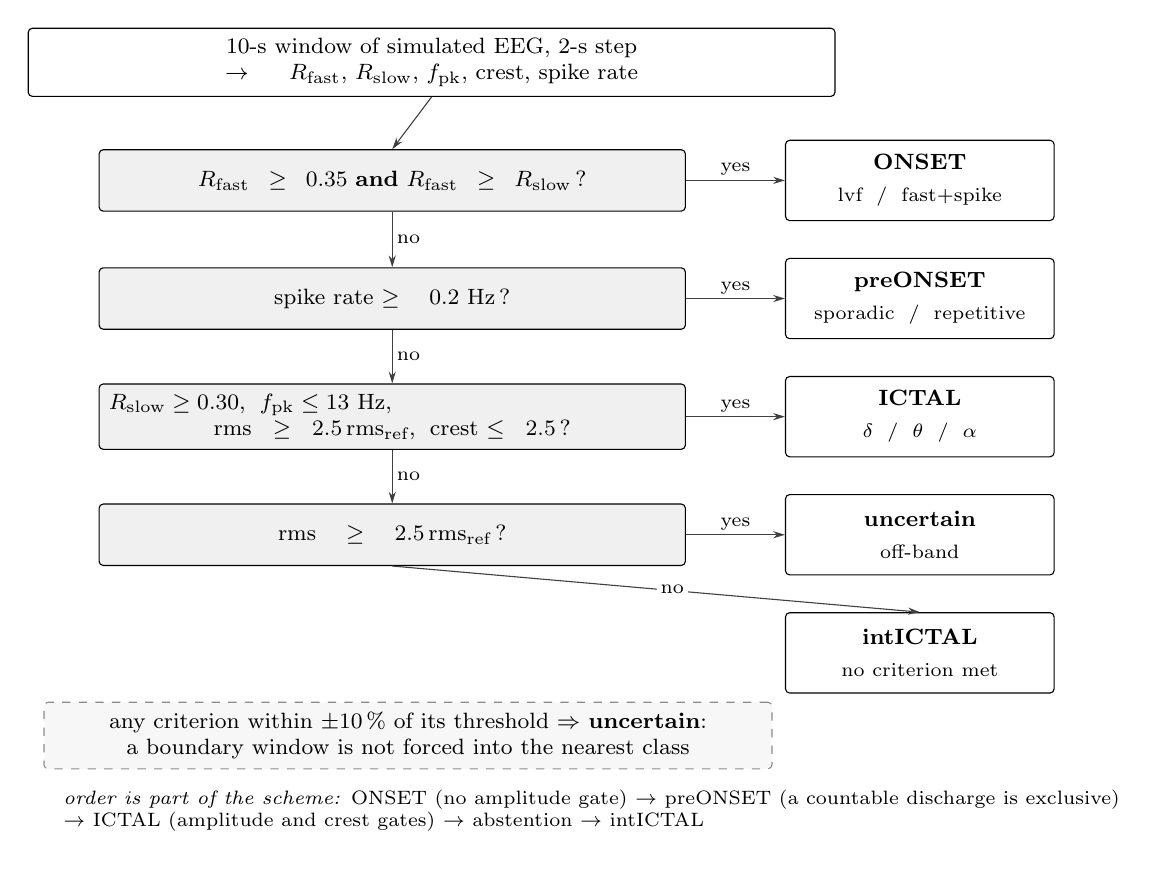
\begin{tikzpicture}[
  font=\footnotesize,
  box/.style   = {draw, line width=0.4pt, rounded corners=1.5pt,
                  align=center, inner sep=3.5pt, minimum height=0.78cm},
  dec/.style   = {box, fill=black!6, text width=7.2cm},
  leaf/.style  = {box, fill=white, text width=3.2cm, minimum height=1.02cm, inner sep=3pt},
  arr/.style   = {-{Stealth[length=1.5mm,width=0.9mm]},
                  line width=0.4pt, draw=black!75},
  lbl/.style   = {font=\scriptsize, inner sep=1.5pt, fill=white}
]

% ---------------- 坐标 ----------------
\def\lx{6.70}     % 叶节点 x
\def\dy{-1.50}    % 层间距

% ---------------- 输入 ----------------
\node[box, text width=10.0cm] (input) at (0.5,0)
  {10-s window of simulated EEG, 2-s step $\;\rightarrow\;$
   $R_{\text{fast}}$, $R_{\text{slow}}$, $f_{\text{pk}}$, crest, spike rate};

% ---------------- 判定链 ----------------
\node[dec] (d1) at (0,\dy)
  {$R_{\text{fast}}\ge 0.35$ \textbf{and} $R_{\text{fast}}\ge R_{\text{slow}}$\,?};
\node[dec] (d2) at (0,2*\dy)
  {spike rate $\ge 0.2$~Hz\,?};
\node[dec] (d3) at (0,3*\dy)
  {$R_{\text{slow}}\ge 0.30$, \;$f_{\text{pk}}\le 13$~Hz,\newline
   $\mathrm{rms}\ge 2.5\,\mathrm{rms}_{\text{ref}}$, \;crest $\le 2.5$\,?};
\node[dec] (d4) at (0,4*\dy)
  {$\mathrm{rms}\ge 2.5\,\mathrm{rms}_{\text{ref}}$\,?};

% ---------------- 叶节点 ----------------
\node[leaf] (l1) at (\lx,\dy)
  {\textbf{ONSET}\\[2pt]{\scriptsize lvf \;/\; fast+spike}};
\node[leaf] (l2) at (\lx,2*\dy)
  {\textbf{preONSET}\\[2pt]{\scriptsize sporadic \;/\; repetitive}};
\node[leaf] (l3) at (\lx,3*\dy)
  {\textbf{ICTAL}\\[2pt]{\scriptsize $\delta$ \;/\; $\theta$ \;/\; $\alpha$}};
\node[leaf] (l4) at (\lx,4*\dy)
  {\textbf{uncertain}\\[2pt]{\scriptsize off-band}};
\node[leaf] (l5) at (\lx,5*\dy)
  {\textbf{intICTAL}\\[2pt]{\scriptsize no criterion met}};

% ---------------- 连线 ----------------
\draw[arr] (input.south) -- (d1.north);
\draw[arr] (d1.south) -- node[lbl,right] {no} (d2.north);
\draw[arr] (d2.south) -- node[lbl,right] {no} (d3.north);
\draw[arr] (d3.south) -- node[lbl,right] {no} (d4.north);
\draw[arr] (d4.south) -- node[lbl,right] {no} (l5.north);

\draw[arr] (d1.east) -- node[lbl,above] {yes} (l1.west);
\draw[arr] (d2.east) -- node[lbl,above] {yes} (l2.west);
\draw[arr] (d3.east) -- node[lbl,above] {yes} (l3.west);
\draw[arr] (d4.east) -- node[lbl,above] {yes} (l4.west);

% ---------------- 说明框 ----------------
\node[box, draw=black!45, dashed, text width=9.0cm, fill=black!3]
  (note) at (0.2,5*\dy-1.05)
  {any criterion within $\pm10\,\%$ of its threshold $\Rightarrow$ \textbf{uncertain}:
   a boundary window is not forced into the nearest class};

% ---------------- 次序注 ----------------
\node[font=\scriptsize, align=left, anchor=north west] at (-4.3,5*\dy-1.62)
  {\textit{order is part of the scheme:} ONSET (no amplitude gate) $\rightarrow$
   preONSET (a countable discharge is exclusive)\\
   $\rightarrow$ ICTAL (amplitude and crest gates) $\rightarrow$ abstention $\rightarrow$ intICTAL};

\end{tikzpicture}
\end{document}
